\subsection{Contextualização do Ambiente}\label{sec::desc_contex}

A usina hidrelétrica de Jirau é do tipo fio d'água, na qual são utilizadas turbinas do tipo bulbo de eixo horizontal. Como a geração de energia depende da altura da queda
d'água e da vazão do rio, as turbinas do tipo bulbo utilizam uma grande vazão de
água para produzirem energia elétrica suficiente. A figura
\ref{fig::bulb_turbine} e a tabela \ref{tab::bulb_turbine} ilustram uma turbina
do tipo bulbo e o grandes dutos necessários para comportar o grande volume de água que passa através da turbina. 
 
\begin{figure}[h!]	
	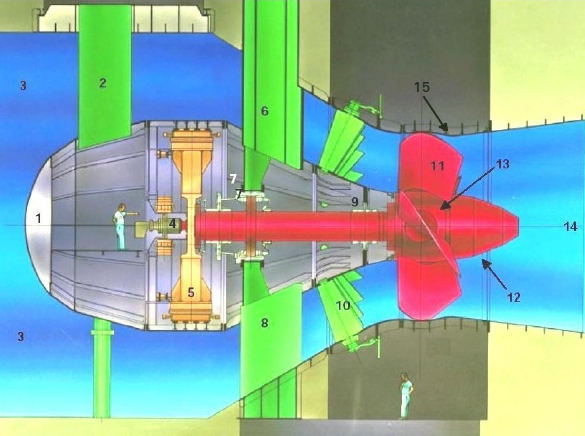
\includegraphics[width=\columnwidth]{figs/intro/bulb_turbine2}
	\caption{Ilustração de uma turbina do tipo bulbo.}
	\label{fig::bulb_turbine}
\end{figure}

\begin{center}
\begin{tabular}{  c | c  }
  \hline
  \textbf{Número} & \textbf{Componente} \\ \hline
  1 & Nariz do bulbo \\ \hline
  2 & Tubo de acesso ao gerador  \\ \hline
  3 & Câmara de adução  \\ \hline
  4 & Cabeçote Kaplan  \\ \hline
  5 & Gerador Síncrono  \\ \hline
  6 e 8 & Estrutura de sustentação \\ \hline
  6 & Tubo de acesso à turbina \\ \hline
  7 e 9 & Mancais Combinado e Guia \\ \hline
  10 & Distribuidor \\ \hline
  11 & Pás do Rotor \\ \hline
  12 & Cone ou Ogiva \\ \hline
  13 & Cubo \\ \hline
  14 & Tubo de sucção/descarga \\ \hline
  15 & Aro Câmara \\
  \hline
\end{tabular}
\captionof{table}{Componentes principais de uma turbina tipo bulbo}
%\caption{Componentes principais de uma turbina tipo bulbo}
\label{tab::bulb_turbine}
\end{center}



Atualmente, caso seja necessário algum reparo ou inspeção na turbina, é necessário que se interrompa o fluxo de água e que 
toda a água em seu interior seja drenada. Para manutenção do rotor, existe uma escotilha de acesso de diâmetro limitado. Entretanto, caso deseje-se realizar 
a metalização de pás já instaladas, utilizando-se os processos atuais, é
necessária a retirada de todo o aro câmara, desmontagem completa do rotor e logística de transporte das pás até o local
onde a metalização será realizada. Essa operação, caso necessite ser realizada, demandaria a mobilização
de diversas equipes de manutenção, operação de pórtico rolante e transporte,
além de impossibilitar a utilização da turbina durante várias semanas.
No contexto da solução proposta, os pontos de interesse da turbina são:

\begin{itemize}
  \item Hélice e pás;
  \item Aro Câmara e regiões adjacentes;
  \item Escotilhas de acesso;
  \item Tubo de Sucção;
  \item Infraestrutura disponível
\end{itemize} 

\subsubsection{Hélice e pás}
 
O rotor ou hélice da turbina é constituído do cubo, as pás e o cone. 
Nas turbinas da usina de Jirau, cada pá mede, aproximadamente, 2,5m de altura e
3m de largura. A partir do interior da turbina, todas as superfícies da pá são
alcançáveis, com exceção da borda e do lip da pá. O único ponto de acesso à
essa regiâo é por meio da escotilha superior de acesso. A figura
\ref{fig::blade_rijeza} exemplifica uma pá do rotor presente na usina de Jirau recém metalizada no galpão da Rijeza.

\begin{figure}[h!]	
	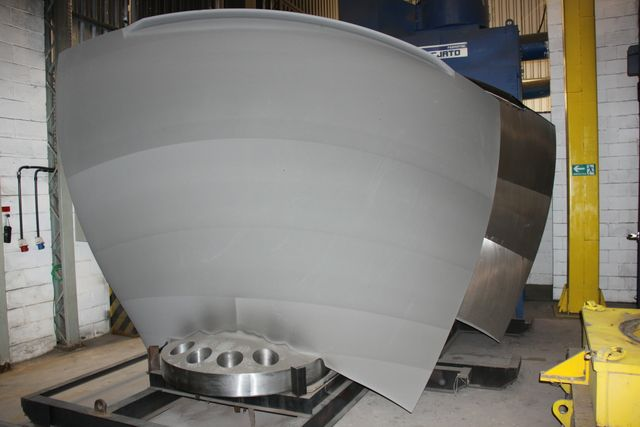
\includegraphics[width=\columnwidth]{figs/viagem/2015_04_28/Rijeza/img_4887}
	\caption{Pá do rotor recém metalizada.}
	\label{fig::blade_rijeza}
\end{figure}

A angulação de cada pá em relação ao fluxo d'água pode ser alterado em 29$^o$,
14.5$^o$ para cada lado a partir da posição inicial, não havendo sobreposição
entre as pás, como ilustrado na figura \ref{fig::blades_angle}.
Essa angulação pode ser explorada para otimizar o espaço de trabalho necessário
para o processamento da pá e também influencia o acesso à região
entre o distribuidor e o rotor, uma vez que não existe acesso pela montante da turbina. A posição do 
rotor também pode ser manualmente alterada, possibilitando 
que o mesmo seja girado em ambas as direções e sem limite de revoluções. Entretanto, essa operação 
é uma tarefa imprecisa e envolve um certo risco às pessoas que a realizam. Sendo
assim, a solução proposta deve otimizar o número de rotações necessárias para o processamento de todas as pás.

\begin{figure}[h!]	
	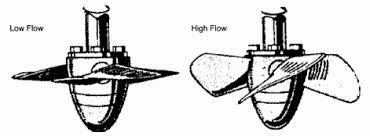
\includegraphics[width=\columnwidth]{figs/intro/blades_angle}
	\caption{Exemplo de limites de rotação das pás do rotor.}
	\label{fig::blades_angle}
\end{figure}

\subsubsection{Aro Câmara e regiões adjacentes}

O aro câmara, assim como o a região próxima ao distribuidor e também ao tubo de
sucção possuem superfícies metálicas. Essa característica possibilita a
exploração de soluções de fixação magnética.

Somente a região compreendida pelo aro câmara é plana e tendo como agravante a presença do distribuidor na região à 
montante ao rotor. É necessário que a inclinação presente nessas superfícies seja contabilizada e uma solução eficiente 
de apoio ou plano elevado seja desenvolvida caso haja necessidade de fixação de alguma parte do sistema. Atualmente todo 
o trabalho é realizado por meio da montagem de andaimes ancorados por cordas. A
figura \ref{fig::andaime} ilustra uma estrutura utilizada no modo de inspeção e
manutenção atuais.

\begin{figure}[h!]	
	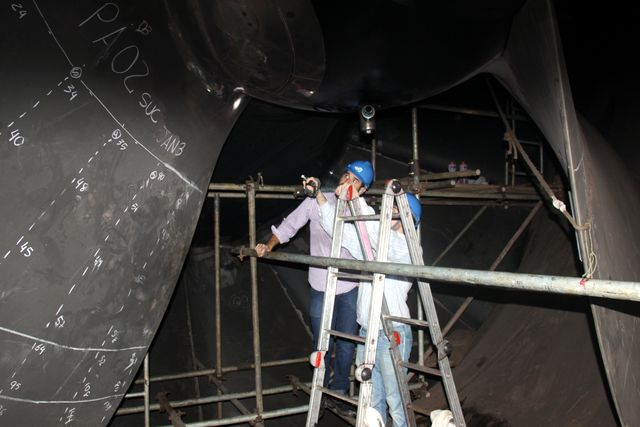
\includegraphics[width=\columnwidth]{figs/viagem/2015_04_28/UG/img_4969}
	\caption{Andaime montado no interior da turbina e ancorado por cordas}
	\label{fig::andaime}
\end{figure}

 
\subsubsection{Escotilhas de acesso}
O acesso à turbina se dá por duas escotilhas, uma inferior, localizada no ínicio do tubo de sucção 
próxima ao aro câmara e outra superior, localizada na parte superior do aro câmara.

A escotilha inferior é o acesso utilizado para a entrada de pessoas na turbina e todo 
material utilizado para reparos é transportado através dessa escotilha. Na usina de Jirau existem dois 
tipos de escotilha de acesso inferior, sendo a menor delas possuindo 80cm de diâmetro. 

A escotilha superior é utilizada, principalmente, para a inspeção visual do
estado dos Lips das pás.
O diâmetro do acesso superior é de aproximadamente $35.7cm$, limitando as
dimensões dos equipamentos que podem ser transportados através da escotilha. As figuras \ref{fig::esc_sup_ext} e
\ref{fig::esc_sup_int} ilustram o acesso à escotilha superior pelo exterior ao
aro câmara e a visão pelo interior da turbina,
respectivamente.

\begin{figure}[h!]	
	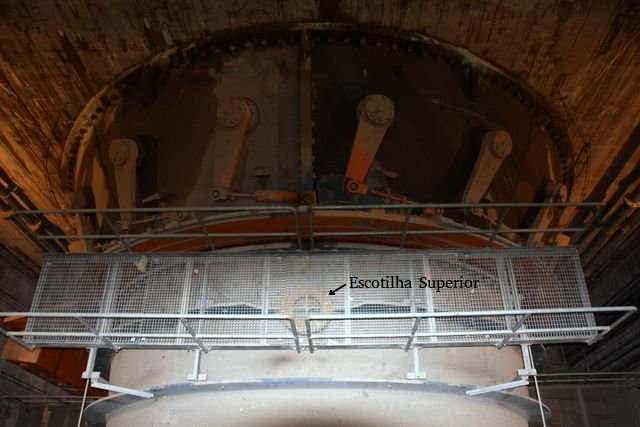
\includegraphics[width=\columnwidth]{figs/viagem/2015_04_28/UG/img_4979_mod}
	\caption{Vista da escotilha superior pelo exterior do aro câmara}
	\label{fig::esc_sup_ext}
\end{figure}

\begin{figure}[h!]	
	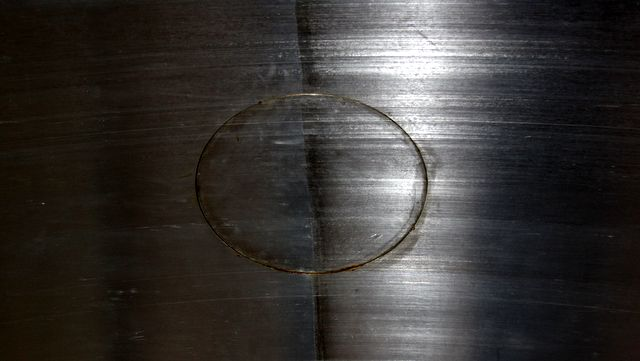
\includegraphics[width=\columnwidth]{figs/viagem/2015_04_28/UG/img_4982}
	\caption{Vista da escotilha superior pelo interior do aro câmara}
	\label{fig::esc_sup_int}
\end{figure}

\subsubsection{Tubo de sucção}

Ao final do tubo de descarga está localizado o vão dos stoplogs 
de jusante ou da comporta vagão e, em seguida, o leito do rio. %Caso os stoplogs 
%não estejam inseridos, existe um vão de acesso de pelo menos 10m de largura. O 
%fluxo de água pode ser controlado pela abertura do distribuidor, criando assim 
%um acesso extra para um sistema submarino. A figura \ref{fig::tubo_suc}
%exemplifica a magnitude do tamanho do acesso, deixando claro que o limitante de
%tamanho do sistema para a utilização desse acesso é o vão de entrada do
% stoplog, ilustrado na figura \ref{fig::stoplog}. Outra alternativa é utilizar um
%guindaste e submergir o sistema pelo próprio rio, entretanto o sistema ficaria
%sujeito as condições do ambiente.

\begin{figure}[H]	
	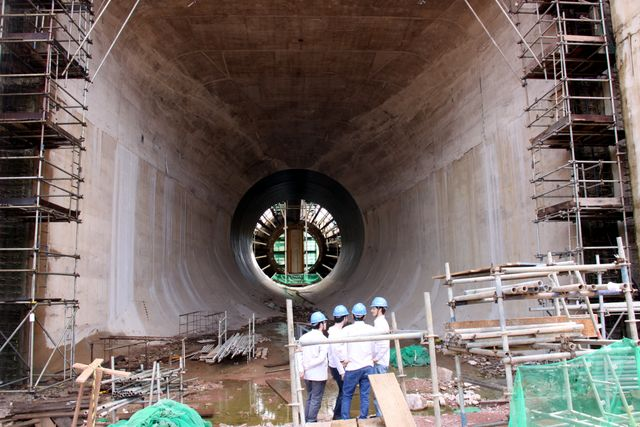
\includegraphics[width=\columnwidth]{figs/viagem/2015_04_30/Vao/img_5086}
	\caption{Abertura do tubo de sucção para o leito do rio, em fase de
	construção.}
	\label{fig::tubo_suc}
\end{figure}

\subsubsection{Infraestrutura disponível}
É importante ressaltar a infraestrutura dísponível para o desenvolvimento da solução. 
Após secar a turbina, é possível a disponibilização de energia elétrica e ar
comprimo em seu interior, ambos importantes para o processo de metalização. Outro fator 
importante é a presença de um pórtico rolante que tem acesso até o andar diretamente 
inferior ao aro câmara, posicionando todo o equipamento necessário nas proximidades 
da escotilha de acesso inferior. É possível também o acesso direto, por meio de pórtico, 
à escotilha superior.

\begin{figure}[h!]	
	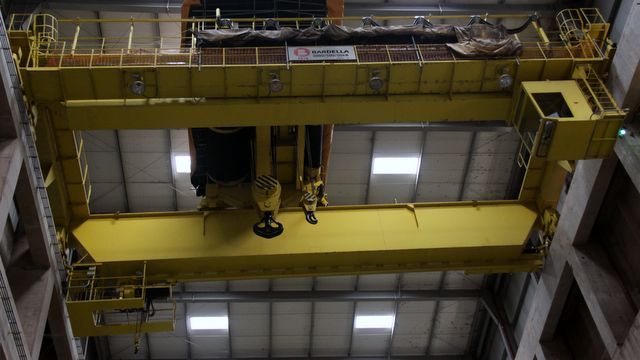
\includegraphics[width=\columnwidth]{figs/viagem/2015_04_28/UG/img_4989}
	\caption{Pórtico rolante com acesso ao exterior do aro câmara}
	\label{fig::portico}
\end{figure}


O ambiente pode ser resumidamente caracterizado pelas dimensões das pás,
elemento a ser processado; características do aro câmara, estrutura que limita o
espaço de trabalho do robô; e pelos acessos nos quais o sistema terá que
utilizar.

\begin{itemize}
  \item \textbf{Pás do rotor} - Material aço inox 420. Dimensões 2.5 x 2.5 m de superfície;
  \item \textbf{Aro Câmara} - estrutura cilíndrica com raio de 3.95 m e
  superfície metálica;
  \item \textbf{Acessos}: 
  	\begin{itemize}
    	\item Escotilha superior - 35 cm de diâmetro;
  		\item Escotilha inferior - 80 cm de diâmetro;
  		\item Tubo de descarga - 20 x 20 m, porém acessado pelo rio. 
  	\end{itemize}
\end{itemize}






